\section{Analytic Provenance}
Analytic provenance research tries to understand a user's reasoning process by examining their interactions with a visual analytic system. Visual analytics is the science of analytical reasoning facilitated by interactive visual interfaces \cite{Thomas2005}. The key role of visual analytics is to support analysts to derive insight from massive amounts of data and to make decision based on the derived knowledge. However, not only is the extracted knowledge important, but the analysis process that led to that knowledge and the rationale underlying the analysis are also of great significance \cite{North2011, Heer2008}.

In 1996, Shneiderman already noticed the importance of studying user interactions in information visualisation by classifying \textit{history} as one of the seven tasks in his \textit{Task by Data Type Taxonomy} \cite{Shneiderman1996}. According to Shneiderman, information visualisation systems need to support users to review previous actions and correct mistakes because the information exploration process is typically long and complex. Since then, there has been more research on exploration history and analytic provenance in visualisation and related fields. In May 2011, the first workshop dedicated to analytic provenance was held in \textit{CHI 2011} conference to develop a research agenda to better study analytic provenance and a call to action for further research. In that workshop, the following definition of analytic provenance was proposed, ``the area of research that focuses on understanding a user's reasoning process through the study of their interactions with a visualisation is called Analytic Provenance'' \cite[p.33]{North2011}. Besides understanding the user's reasoning process, many benefits can also be gained from analytic provenance such as recalling the analysis process, reusing performed analyses, supporting evidence in constructing the reasoning process, and facilitating collaboration between colleagues including dissemination, discussion and presentation (Section \ref{sub:utilisation}). 

Typically, an \textit{analytic provenance aware} system consists of three stages: capturing the provenance of the analysis process, visualising the captured information, and utilising the visualised provenance. As a result, we characterise the literature of analytic provenance by these stages.

why this model is used to support sensemaking
Brehmer2013: multi-level typology of abstract visualization tasks addressing 3 aspects why the task is performed, how the task is performed, and what are the inputs and outputs of the task. 3 levels for why.

other model to characterize actions

In contrast, user-oriented taxonomies typically charac- terize high-level human cognitive tasks or visual percep-
tual behaviors.25–28 For example, Amar et al25 have come up with 10 basic task types describing various users’ needs in information analysis. Existing user-oriented taxonomies often characterize behavior at granulari- ties which correspond closely to the Task or Sub-task tiers in our characterization. Compared to the previous taxonomies, our work is unique in identifying the Action tier, a granularity of activity that bridges the semantic gap between high-level human cognitive activity and low-level user visual interaction events.


\subsection{Capturing Analytic Provenance}
% What to capture? Gotz and Zhou model. Why this model? Use those four tiers to review.
The first step in capturing analytic provenance is to decide what kind of information needs to be captured. Does the system capture low-level user interactions, or high-level user intentions, or both of them? The decision may depend upon how the system subsequently uses the captured information.

%TODO: May need an example for this model and a picture with 4 models.
Based on an empirical study, Gotz and Zhou \cite{Gotz2009} characterise visual analytic activities at multiple levels of granularity according to the semantic richness of these activities: the top-level \textit{tasks} (high-level analytic goals), the high-level \textit{sub-tasks} (more concrete sub-goals to fulfil the goal), the low-level \textit{actions} (detailed analytic steps to achieve the sub-goal such as filtering or sorting data) and the bottom-level \textit{events} (the actual interactions need to perform such as mouse-clicks or keystrokes). Figure \ref{fig:Gotz-Zhou-Model} illustrates the model and an example scenario.

\begin{figure}[ht]
\centering
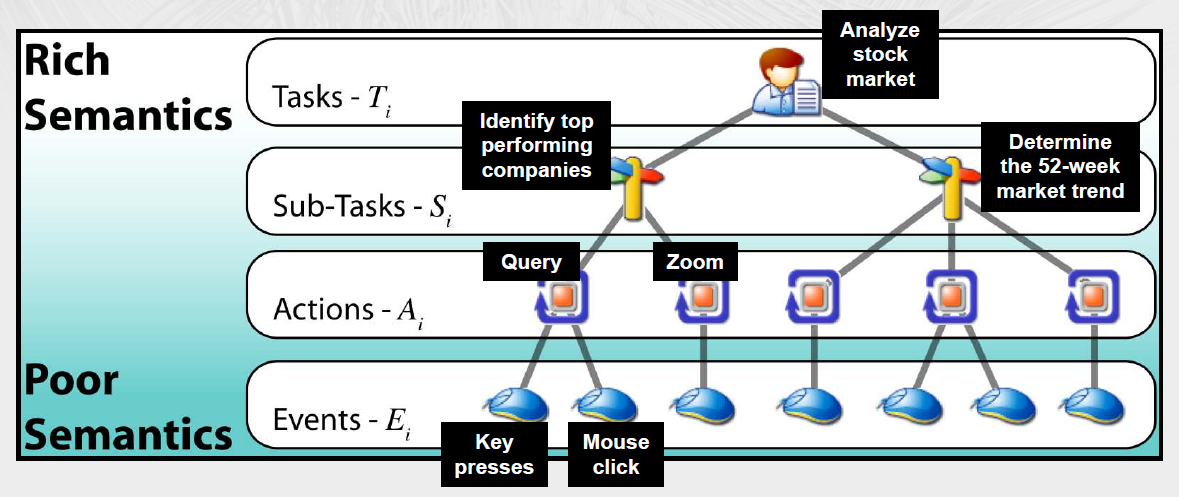
\includegraphics[width=\columnwidth]{Gotz-Zhou-Model-Example.png}
\caption{Illustration of the Gotz and Zhou model \cite{Gotz2009} with an example in business environment. One possible analysis task is to analyse the stock market to invest. Two proposed sub-tasks are identifying the top performing companies and finding the trend of the market this year. To accomplish the first sub-task, the analyst queries top 50 highest profit companies, which requires clicking on the query button and typing '50'. All these task, sub-tasks, actions and events are represented in the model.}
\label{fig:Gotz-Zhou-Model}
\end{figure}

Following this characterisation, a system can capture the information corresponding to one or many tiers. We describe the existing work of capturing provenance of each tier below.


%Gotz and Zhou} characterise visual analytics activities at four levels of granularity: tasks, sub-tasks, actions and events. A \textit{task} is a high-level analyticand \textit{sub-tasks} represent high-level goals and plans of the analyst to solve a particular task. These two tiers are rich-semantic and domain specific. The third tier, \textit{actions}, represents detailed steps that the analyst uses to implement the proposed plan; for instance, sort data or zoom view. These actions are rich-semantic and sufficient generic to use as the building blocks of provenance representation. Whereas, the last tier, \textit{events}, contains least semantics and maps to user interactions such as mouse movements and keystrokes. 

%TODO: Need to mention some other taxonomies? Why choose this model?
%
%\subsubsection{Capturing Bottom-Level Events}
%Glass Box \cite{Cowley2006} can record a great deal of low-level information including keyboard/mouse events, window events, file open and save events, copy/paste events, and so on. Its objective is to capture, archive and retrieve intelligence analysis activities.
%
%%Critique
%There is not much research on capturing events because it is relatively easy and limitedly useful. Simply capturing these events alone does not provide sufficient information to understand their purpose and rationale. For example, we know that a \textit{mouse click} is captured; however, what the purpose of that click was (e.g., to sort the data?), and why the user performed that click (e.g., to find an interesting pattern from the data?) are unknown. Commonly, when analysing data with a visualisation, an analyst needs to perform many operations with trials and errors to find the answer to the problem. In that case, a series of poor-semantic and bottom-level events makes it more difficult for the analyst to recall what has been done. Therefore, more meaningful interactions also need to be captured. 
%
%\subsubsection{Capturing Low-Level Actions}
%\paragraph{Taxonomy of Actions}
%Actions in the action tier are both semantic and generic across different visual analytic systems, thus are commonly used as the semantic building blocks for the provenance of derived insight \cite{Groth2006, Shrinivasan2008, Gotz2009}. Gotz and Zhou \cite{Gotz2009} provide a taxonomy of actions that contains the most common analytic operations in many visual analytics systems they observed. The taxonomy classifies actions, based on their intention, into three groups: \textit{exploration} actions (e.g., \textit{filter} the data according to a condition), \textit{insight} actions (e.g., \textit{bookmark} the current visualisation), and \textit{meta} actions (e.g., \textit{undo/redo} a performed action). 
%
%Considering an example to distinguish between capturing meaningful actions and less-meaningful events. The action \textit{zoom-in} has an intention of increasing the details of the display area, and thus can be used either to reduce the focus area of a map or to refine the display time range of a timeline, in a semantically equivalent manner. Moreover, this action could be accomplished by three different events: scrolling the mouse, pressing the combination of Ctrl and plus (+), and tapping on a smart device. Recording only the event; for instance, scrolling the mouse, is not sufficient to know whether its action is zoom or just a common scroll in a text editor.
%
%\paragraph{Automatically Capturing Low-Level Actions}
%During the course of analysis with a visualisation, all user interactions can be systematically recorded. The visual exploration process can be modelled using \textit{graph} metaphor. Nodes in the graph represent \textit{states} of the application and edges represent \textit{actions} that transform one state into the other state. Considering an  example of \textit{bar-chart} visualisation, states are all the necessary information allowing to reconstruct the captured chart such as the \textit{dataset} and the \textit{colour map}; while an action could be \textit{sorting data}. The system can support \textit{undo} to revisit to a previous state; and if a new action is performed at that state, a new branch will be created to store that new line of inquiry. 
%
%Basically, there are two prime strategies to automatically capture the exploration process. One is capturing the initial state and all the performed actions so that they can be rerun to achieve the desired state \cite{Kadivar2009}. Second is simply capturing all visualisation states after each action \cite{Bavoil2005}. The former strategy suffers from potential long running time if the number of actions need to executed is high; while the latter is memory-expensive if a state contain too much information. The later is easier to implement; whereas, the former allows re-applying the analysis process with a different dataset.
%
%%VisTrails \cite{Bavoil2005}, a scientific workflow and provenance management system, logs every single change to the workflow that could affect the final visualisation; for instance, modification of the \textit{opacity parameter} from 0.4 to 1. The 3D molecule viewer described in \cite{Groth2006} captures interactions that alter the observed view including \textit{zoom}, \textit{rotate}, and \textit{translate}.
%
%%\subparagraph{Capture Model}
%%%TODO: rereads the two papaers and adds more details
%%Jankun-Kelly et al. \cite{Jankun-Kelly2007} propose the \textit{P-Set model} to capture and reuse the information within the visualisation process. The model captures visualisation transforms, parameters (p-sets), results and derivations and store them in an XML representation. This model is successful in capturing the changes of parameter values that lead to changes in the visualisation. However, the model cannot capture the user interactions that made the parameters changed.  In another word, the model is appropriate for scientific visualisation where the need to capture the changes of parameter values is more important than the need to capture the actual user interactions.
%%
%%Another model is the \textit{interaction model} \cite{Groth2006}, which is based on directed graphs. Nodes store visualisation parameters and edges represent transitions between the states. The model is extended to include annotation information. Annotations are special nodes that point to the annotated visualisation nodes. 
%
%
%% Implementation notes
%%\paragraph{Implementation}
%%Heer et al. \cite{Heer2008} reviews techniques to capture user interactions, which allow to revisit to any desired state that happened in the past. Using a \textit{graph metaphor} to model the history of actions, where \textit{nodes} depict states and \textit{edges} depict actions that transform one state into another state. If the system captures the user actions (edges), to recover a state, it is needed to rerun all the actions from the beginning node to the current node of the graph. Otherwise, if the system captures the visualisations (nodes), it is straightforward to reload the past state; however, the data required to store all visualisation states may be large.
%\subsubsection{Capturing High-Level Sub-Tasks or User Intentions}
%Typically, high-level sub-tasks can be either inferred from captured low-level actions or directly recorded by users.
%
%\paragraph{Deriving from Captured Actions} When analysts interact with a visual analytics tool, their plans and methods to analyse data could partially be reflected through their interactions with the application. 
%
%\subparagraph{Manual Derivation}
%Dou et al. \cite{Dou2009} conduct a quantitative study to measure how much of a user's reasoning process can be recovered from only the captured user actions. Reasoning results decoded from the interaction logs are compared with the ground-truth reasoning from analysts' interviews; and the results show that 79 per cent of the findings, 60 per cent of the methods and 60 per cent of the strategies could be extracted from manually analysing the interaction logs. This post-analysis approach is domain-specific because ad hoc tools need to be designed to effectively discover some well-known strategies in a particular domain, detecting suspicious activities in wire transactions. Even though reasoning processes are discovered, the interaction analyses occur after the data analyses and thus cannot support analysts in real-time.
%
%\subparagraph{Automatic Derivation}
%Gotz and Zhou use heuristics to automatically infer a sub-task from a series of actions \cite{Gotz2009}. One heuristic suggests that a user solves a sub-task by completing a combination of several exploration actions followed by an insight action. For example, the analyst explores the data by selecting bar-chart as a visualisation technique (\textit{change-metaphor} action), sorting the data according to some indicator (\textit{sort} action), and then annotating (\textit{annotate} action) on the highest column of the chart. The heuristic considers ``annotate'', the insight action, as a signal of deriving insight, or solving a sub-task; and represents that sub-task as a trail of three actions ``change-metaphor - sort - annotate''. However, if the analyst does not annotate or bookmark visualisations, the heuristic cannot derive any sub-tasks. 
%
%%For example, as in Figure \ref{fig:SubTaskRepresentation}, the analyst performs \textit{query}, \textit{filter}, \textit{zoom}, then goes back to the previous query and performs another \textit{filter}, \textit{inspect} and \textit{bookmark} the visualisation. When the analyst performs the bookmark, which is categorised as an insight action, the system automatically represents that bookmark as the result of a trail of exploration and meta (e.g., \textit{revisit}) actions.
%%\begin{figure}[ht]
%%\centering
%%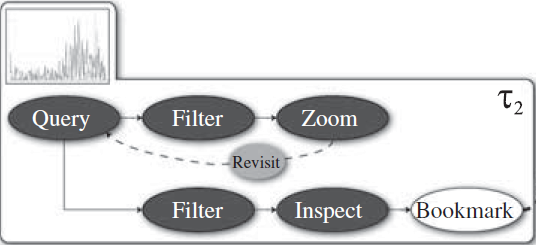
\includegraphics[width=0.5\columnwidth]{SubTaskRepresentation.png}
%%\caption{An example of using heuristics to infer high-level user intention from low-level actions \cite{Gotz2009}. The heuristic assumes that when the analyst bookmarks a visualisation, he/she derives an insight or completes a sub-task in Gotz and Zhou's model. The sub-task is represented as a trail of recently performed exploration and meta actions.}
%%\label{fig:SubTaskRepresentation}
%%\end{figure}
%%Derthick2001
%
%Automatic derivation provides real-time support for users to quickly understand the analysis process. However, because heuristic approach could lead to a misleading user intention, it  should only assist analysts and allow them to correct the derived intention.
%
%\paragraph{Directly Capturing using Annotations}
%Instead of inferring user intentions from low level actions, analysts can manually capture the insight by annotating on the visualisations of interest. Sense.us \cite{Heer2009}, a web site supporting asynchronous collaboration, allows users to annotate on visualisations, and use these annotated visualisations in discussion. GeoTime \cite{Eccles2007}, a geotemporal event visualisation tool, supports embedding hypertext linked visualisations and visual annotations in an analysis story. Annotation can provide more information than simple text and graphics attachment. \textit{Data-aware} annotation detects the subset of data belonging to the annotated area so that the data of interest remains unchanged when new visualisation metaphors are applied for further investigation \cite{Denisovich2005}. Another benefit of data-aware annotation is that statistical values could be automatically generated to add more information such as the mean and the extreme values of selected data items \cite{Chen2010}.
%
%Manual annotation provides high-fidelity; however, users often only take notes of the final state of a visualisation \cite{Gotz2009}. Therefore, intuitive annotation mechanism needs to be designed to encourage users to take notes.
%
%\subsubsection{Capturing Top-Level Tasks}
%Top-level tasks are highly domain-specific; therefore, it's virtually impossible to automatically derive them. The user needs to explicitly write down what the task is before solving the problem. Further enhancement has been made to allow users to document their reasoning processes; for example, recording found interesting patterns about the data, describing their causal relationships, and building a hypothesis based on these found artefacts \cite{Shrinivasan2008, Pike2009a}. This mental model needs to be documented directly onto the same system for effective reasoning rather than keeping tacitly or recording it into an external application such as Microsoft Word (see \cite{Shrinivasan2008} for explanation).
%
%%When the analysis lasts long, the analyst needs to perform a number of operations and probably in a limit of time. Therefore, it is impractical for the analyst to record every insight they found during the analysis. However, this approach provides deeper and more accurate understanding about the captured insights in comparison with the automatic capture approach.
%
%\subsection{Visualising the Captured Information}
%%\begin{figure}[ht]
%%\centering
%%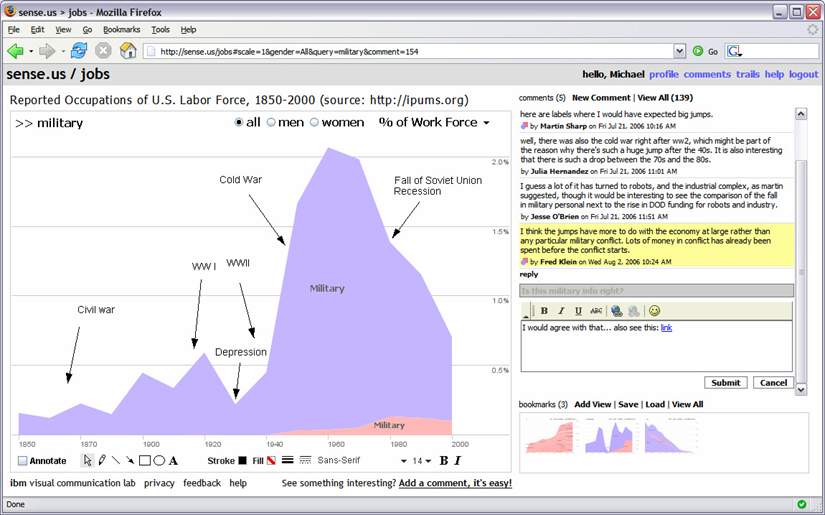
\includegraphics[width=\columnwidth]{Annotation.png}
%%\caption{An example of annotation on visualisations \cite{Heer2009}.}
%%\label{fig:Annotation}
%%\end{figure}
%Typically, events are not visualised because they do not carry much information and the number of events is high. Actions and states (the visual results of the actions) are commonly visualised together to depict the \textit{analysis process}. Sub-tasks and tasks are illustrated in the graphical \textit{reasoning process}. 
%
%\subsubsection{Visualising the Analysis Process}
%Methods of visualising individual actions and states will be discussed, and followed by methods of chaining them together to visualise the entire analysis process. 
%
%\paragraph{Visual Representation of States}
%Conventionally, the space for rendering a state is limited because a small portion of the display area is reserved for provenance information; whereas, the much larger portion is used for data exploration \cite{Shrinivasan2008, Gotz2009, Kadivar2009}. Therefore, a small-scale visualisation of the captured state is popular \cite{Hightower1998} (Figure \ref{fig:thumbnail1}). To recall the affect of the performed action, the miniature can highlight the difference from the previous state \cite{Klemmer2002} (Figure \ref{fig:thumbnail2}), or combine both the former and the latter visualisations corresponding to that action \cite{Kurlander1988} (Figure \ref{fig:thumbnail3}).
%
%\begin{figure}[ht]
%\centering
%\subcaptionbox{The exact miniature of a web-site\cite{Hightower1998}.}{\label{fig:thumbnail1}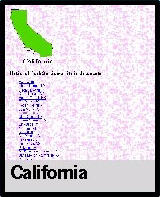
\includegraphics[height=.36\columnwidth]{Thumbnail1.png}} \hspace{0.05cm}
%\subcaptionbox{Each rectangle represents a post-it note. Modified post-it notes are highlighted with green colour \cite{Klemmer2002}.}{\label{fig:thumbnail2}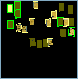
\includegraphics[height=.36\columnwidth]{Thumbnail2.png}} \hspace{0.05cm}
%\subcaptionbox{In a graphical editor, combining the state before the action (above) and the state after the action (bottom) \cite{Kurlander1988}.}{\label{fig:thumbnail3}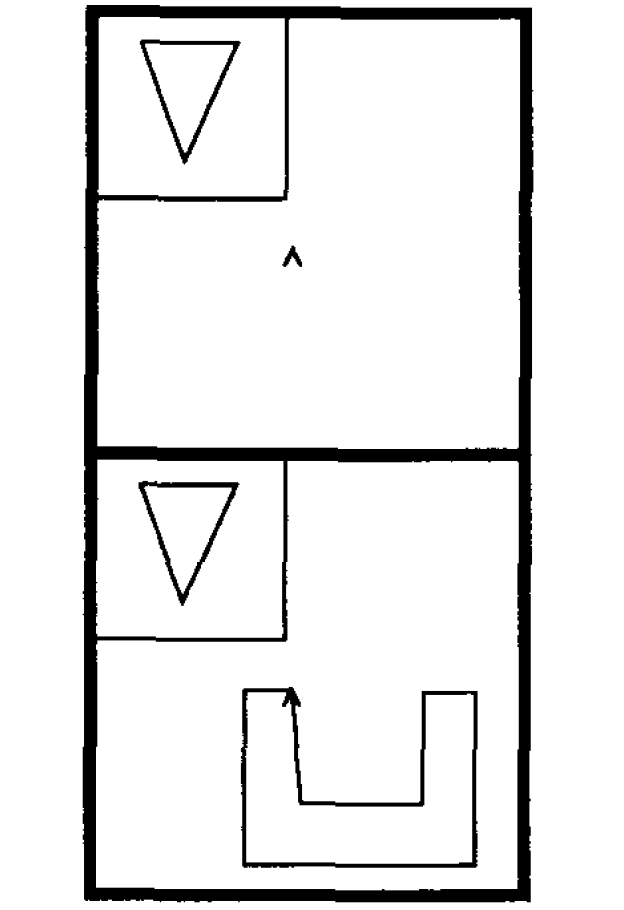
\includegraphics[height=.36\columnwidth]{Thumbnail3.png}}
%\caption{Examples of visual representations of states.}
%\label{fig:State-Respresentation}
%\end{figure}
%
%\paragraph{Visual Representation of Actions}
%Typically, a system supports a certain number of actions; and thus allows using icons to visually distinguish different kinds of actions besides texts \cite{Gotz2009} (Figure \ref{fig:edgeTypes1}). Actions are also commonly represented as edges in a graph to connect two states. Therefore, graph edges can be stylised to reflect the characteristics of the represented actions \cite{Ma1999} (Figure \ref{fig:edgeTypes2}).
%
%\begin{figure}[ht]
%\centering
%\subcaptionbox{Using icons to represent actions including query, filter, change-view and inspect \cite{Gotz2009}.}{\label{fig:edgeTypes1}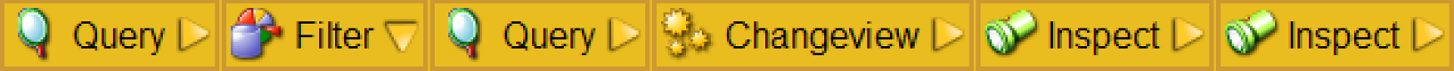
\includegraphics[width=\columnwidth]{EdgeTypes1.png}}
%\subcaptionbox{Using stylish edges to represent actions including changing colour map, rotating, shading, changing opacity, zooming and sampling \cite{Ma1999}.}{\label{fig:edgeTypes2}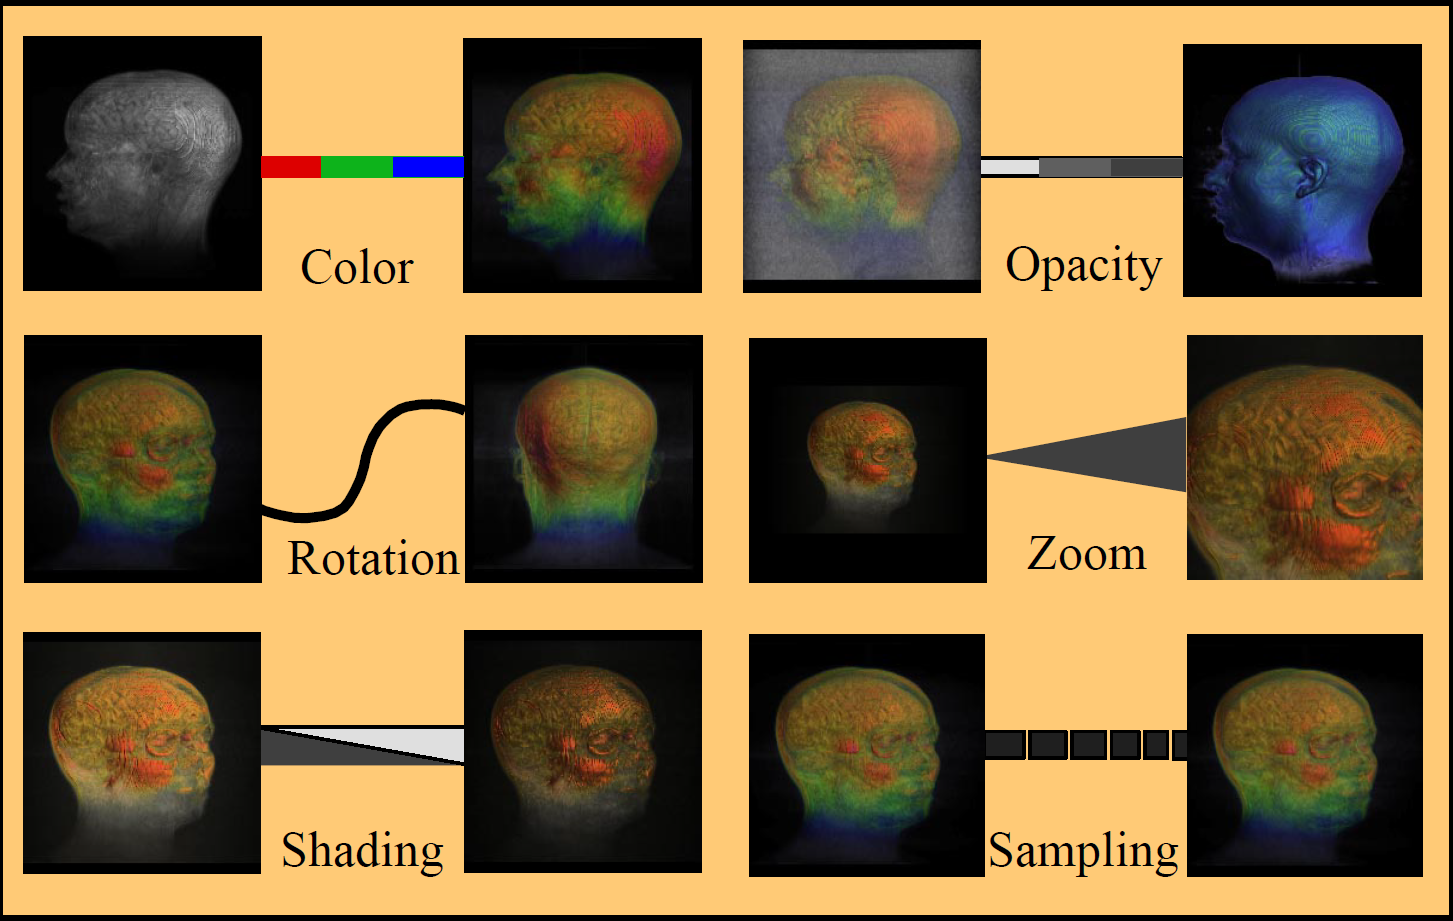
\includegraphics[width=\columnwidth]{EdgeTypes2.png}}
%\caption{Examples of using visual representations of different types of actions.}
%\label{fig:Action-Respresentation}
%\end{figure}
%
%\paragraph{Layout of Actions and States}
%Typically, the system begins with an initial state (node). When the user performs an action, a new node is created for the current state, and a new edge is added to connect the previous node with the current node. Gradually, a string of nodes and edges is built in the chronological order. The system can support revisiting to the previous state. If a new action is performed at that state, a new branch will be forked to store forthcoming actions. Therefore, the analysis process has the layout of a \textit{direct acyclic graph}, or a \textit{tree} if revisited links are not explicitly visualised.
%
%To not distract analysts from the primary data exploration and save space, several techniques have been proposed to reduce the display area of the provenance graph: organising trees in the right horizontal-vertical layout \cite{Shrinivasan2008}, displaying only nodes of the active branch that led to the selected visualisation \cite{Klemmer2002}, allowing graph nodes be expandable/collapsible on demand \cite{Bavoil2005}, supporting zoom-able and pan-able interface \cite{Dunne2012}, and applying distortion techniques to focus on more relevant states \cite{Meng1998}.
%
%The order of actions can be interpreted through the direction of edges in the provenance graph. Moreover, exact time gap between actions can also be measured and visually encoded into the visualisation. VisTrails \cite{Bavoil2005} colour-codes the background of visualisation nodes according to when they are created (Figure \ref{fig:tree1}); and Aruvi \cite{Shrinivasan2008} uses the length of edges to represent the distance in terms of time between two states (Figure \ref{fig:tree2}). This time indication can be updated only when a new node is added, or continuously to reflect the fact that time is always flying. In the latter case, endlessly, background nodes will become lighter and edge lengths will become shorter. This \textit{time-travel} interface is implemented in Visage \cite{Derthick2001}. %TODO: Kai: it's not clear
%
%\begin{figure}[ht]
%\centering
%\subcaptionbox{The darker node refers to the later visualisations \cite{Bavoil2005}.}{\label{fig:tree1}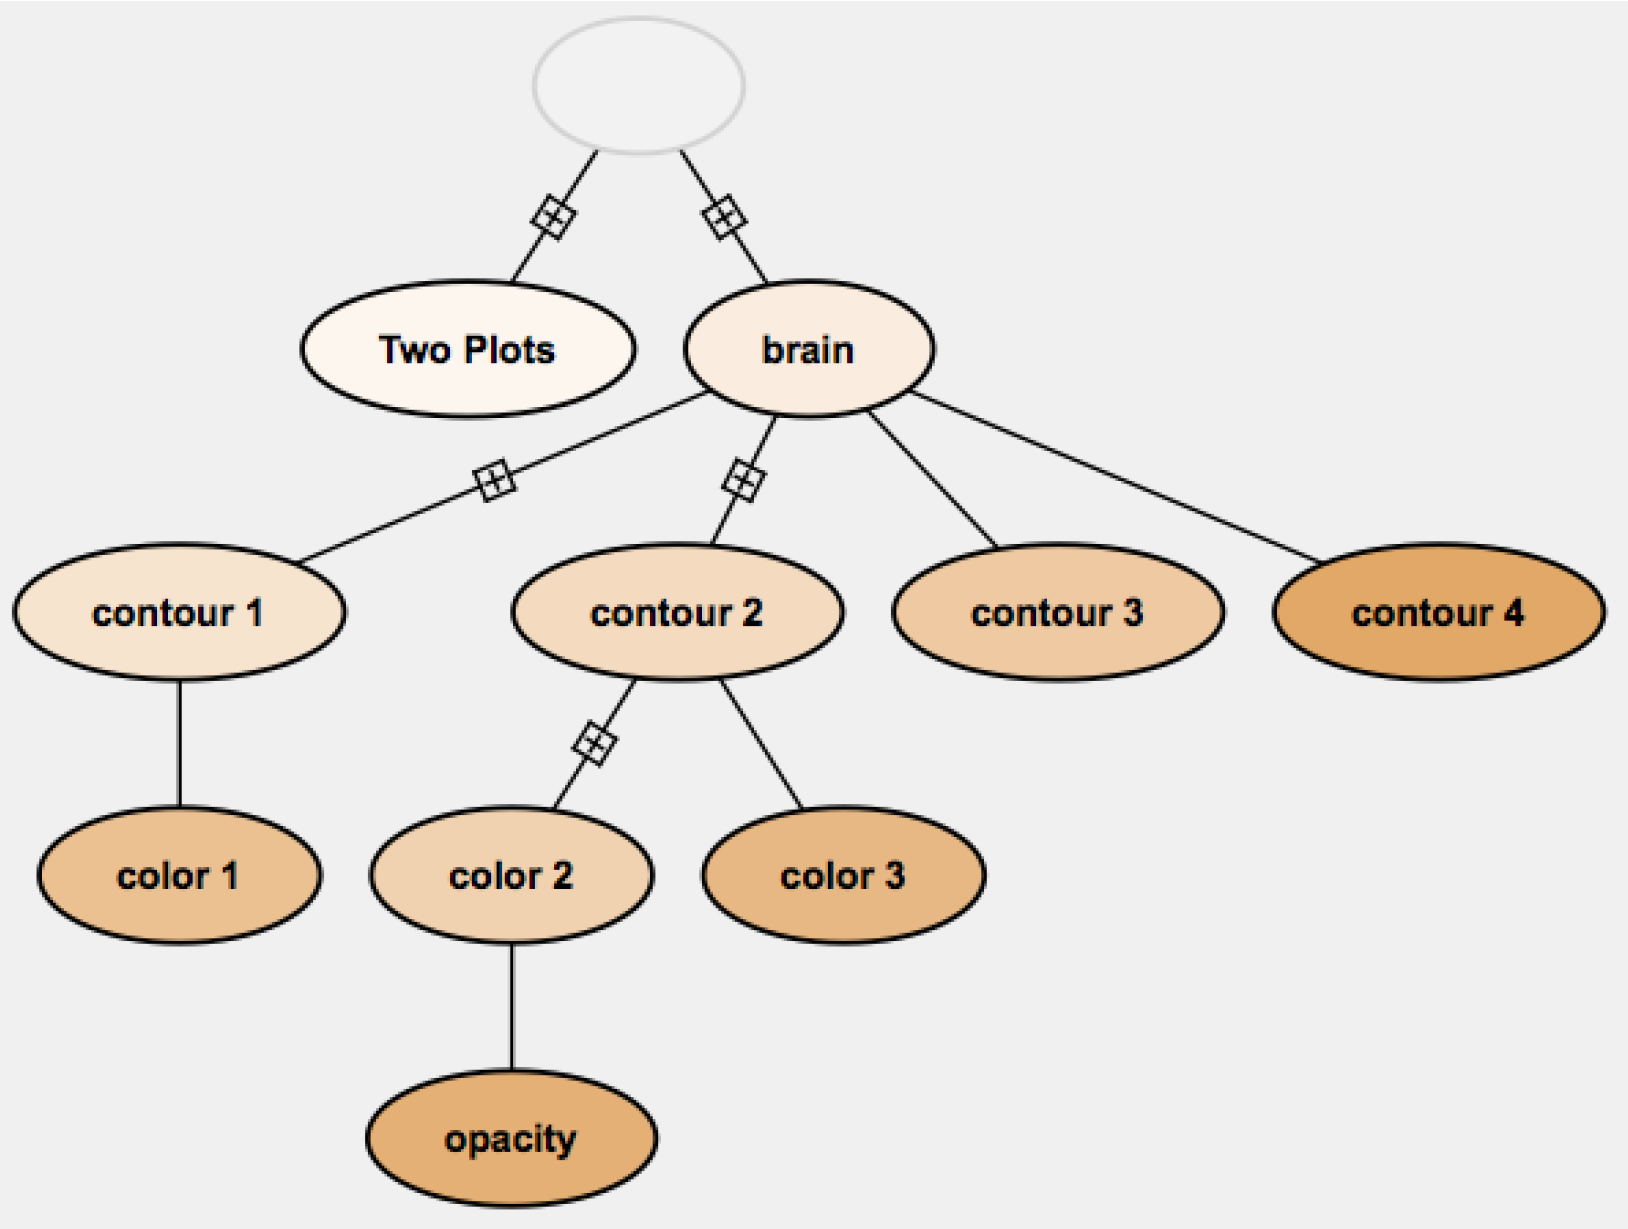
\includegraphics[height=0.21\columnwidth]{Tree-Time-Colour.png}} \hspace{0.1cm}
%\subcaptionbox{The edge length represents time distance between two connecting nodes \cite{Shrinivasan2008}.}{\label{fig:tree2}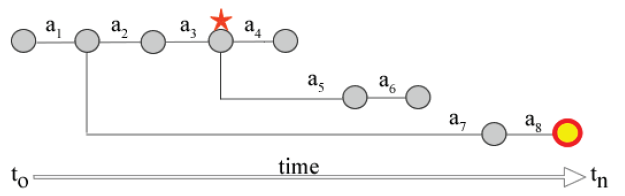
\includegraphics[height=0.21\columnwidth]{Tree-Time-Edge-Length.png}}
%\caption{Examples of encoding time into provenance visualisation.}
%\label{fig:Action-TimeGap}
%\end{figure}
%
%The provenance space can be unified with the data exploration space, where each node of the provenance graph represents a fully interactive visualisation. Zoom-able and pan-able interface needs to be supported to allow users either to focus on the current visualisation  (Figure \ref{fig:focus}) or to observe the entire context of the analysis process (Figure \ref{fig:context}).
%
%\begin{figure}[ht]
%\centering
%\subcaptionbox{Focus view on the active visualisation.}{\label{fig:focus}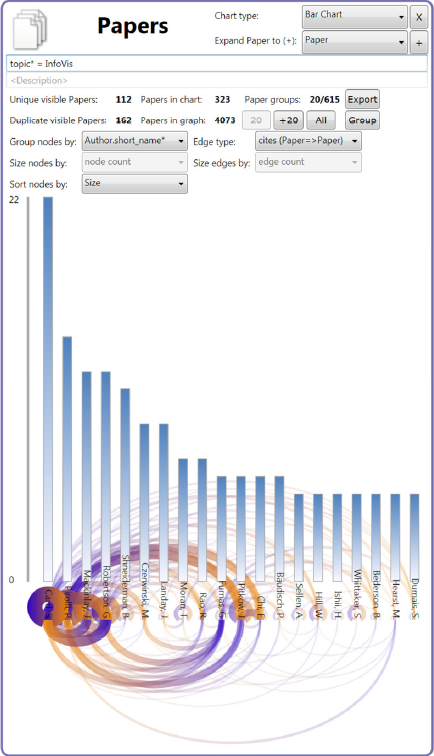
\includegraphics[height=0.57\columnwidth]{GraphTrail-Focus.png}} \hspace{0.1cm}
%\subcaptionbox{Context view to see the overview of what has been done.}{\label{fig:context}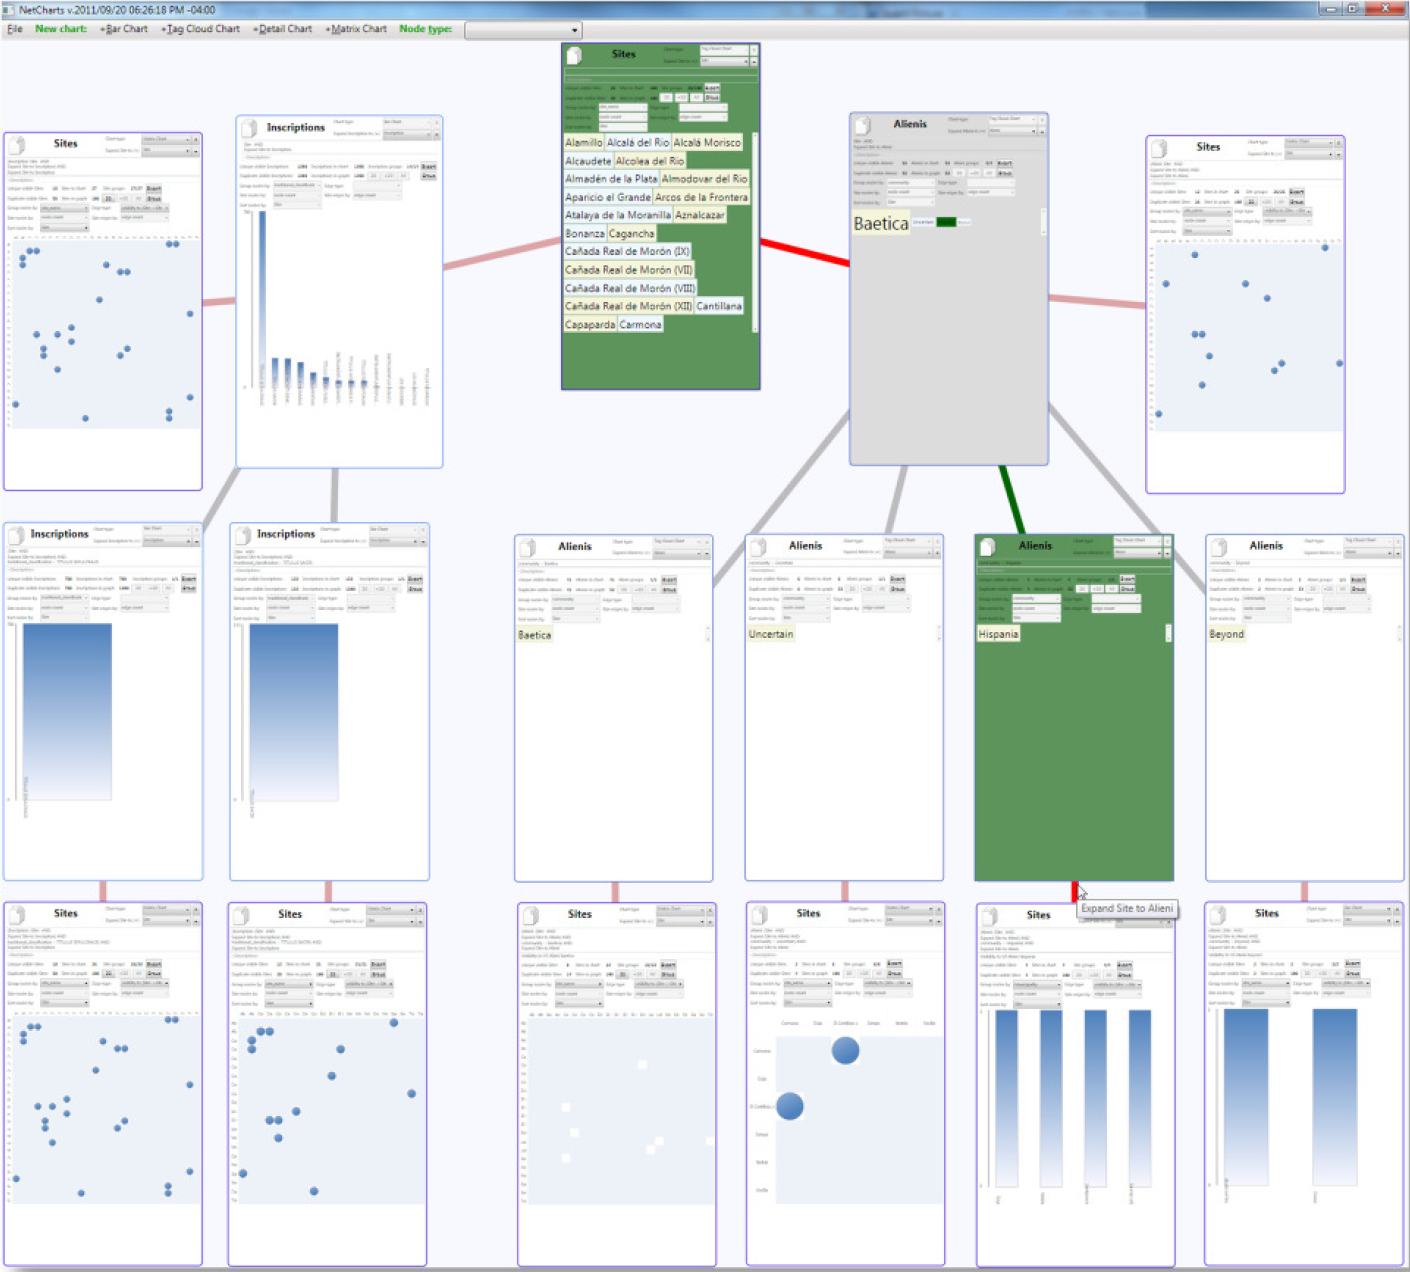
\includegraphics[height=0.57\columnwidth]{GraphTrail-Context.png}}
%\caption{An example of integration of the provenance space into the data exploration space \cite{Dunne2012}.}
%\label{fig:IntegratedView}
%\end{figure}
%
%\subsubsection{Visualising the Reasoning Process}
%\label{sub:reasoningprocess}
%The Aruvi system \cite{Shrinivasan2008} allows analysts to freely compose the reasoning process by using a graphical editor. Users can take note in rectangles or ellipses, and use arrows to connect them. Conventionally, nodes can be referred as \textit{evidence}, \textit{assumptions} or \textit{hypotheses}, and arrows can be referred as \textit{causal relationships}. Nodes in the editor can be linked to the captured visualisations to help explain its reasoning, and these nodes are marked with a star to indicate the existence of the linked visualisations. Instead of using a graphical editor and an implicit convention to map drawing shapes with reasoning artefacts, Scalable Reasoning System \cite{Pike2009a} provides a more formal method to document the reasoning process. A captured visualisation can be dropped to the reasoning space to create a node. The node shows the miniature of the captured visualisation and can be tagged as an \textit{evidence} artefact. An evidence can be converted to a \textit{casual relationship} and its rectangular shape will become an edge. An \textit{assumption} is a free note and can be upgraded as a \textit{hypothesis} when it is supported by an evidence. Figure \ref{fig:ReasoningDocumenting} shows those two examples of reasoning process visualisation.
%
%\begin{figure}[ht]
%\centering
%\subcaptionbox{Using graphical editor to freely construct the mental model \cite{Shrinivasan2008}.}{\label{fig:knowledgeview}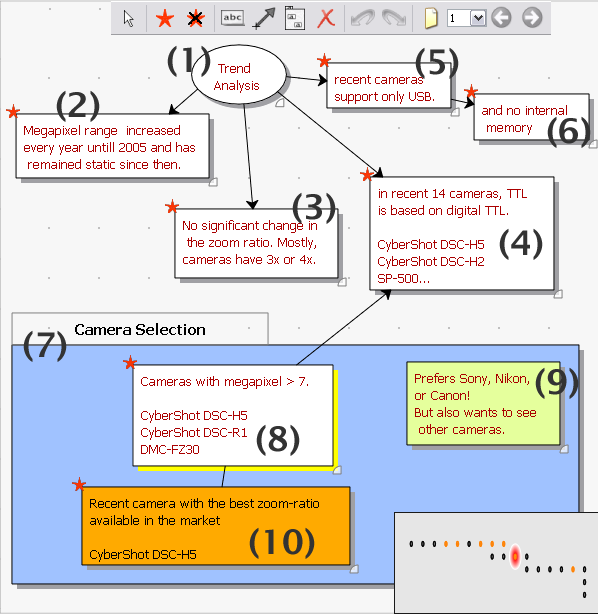
\includegraphics[height=0.39\columnwidth]{Knowledge-View.png}} \hspace{0.1cm}
%\subcaptionbox{A formal reasoning diagram with different types of artefacts: evidence, casual relationship, assumption and hypothesis \cite{Pike2009a}.}{\label{fig:reasoningworkspace}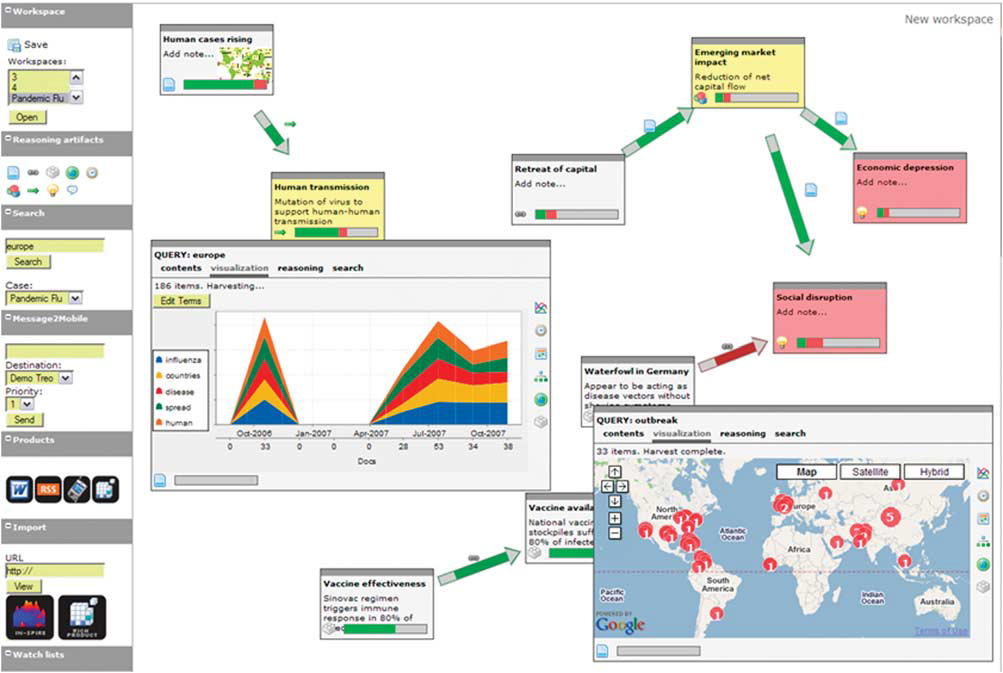
\includegraphics[height=.39\columnwidth]{Reasoning-Workspace.png}}
%\caption{Examples of visualising the reasoning process.}
%\label{fig:ReasoningDocumenting}
%\end{figure}
%
%%\begin{figure}[ht]
%%\centering
%%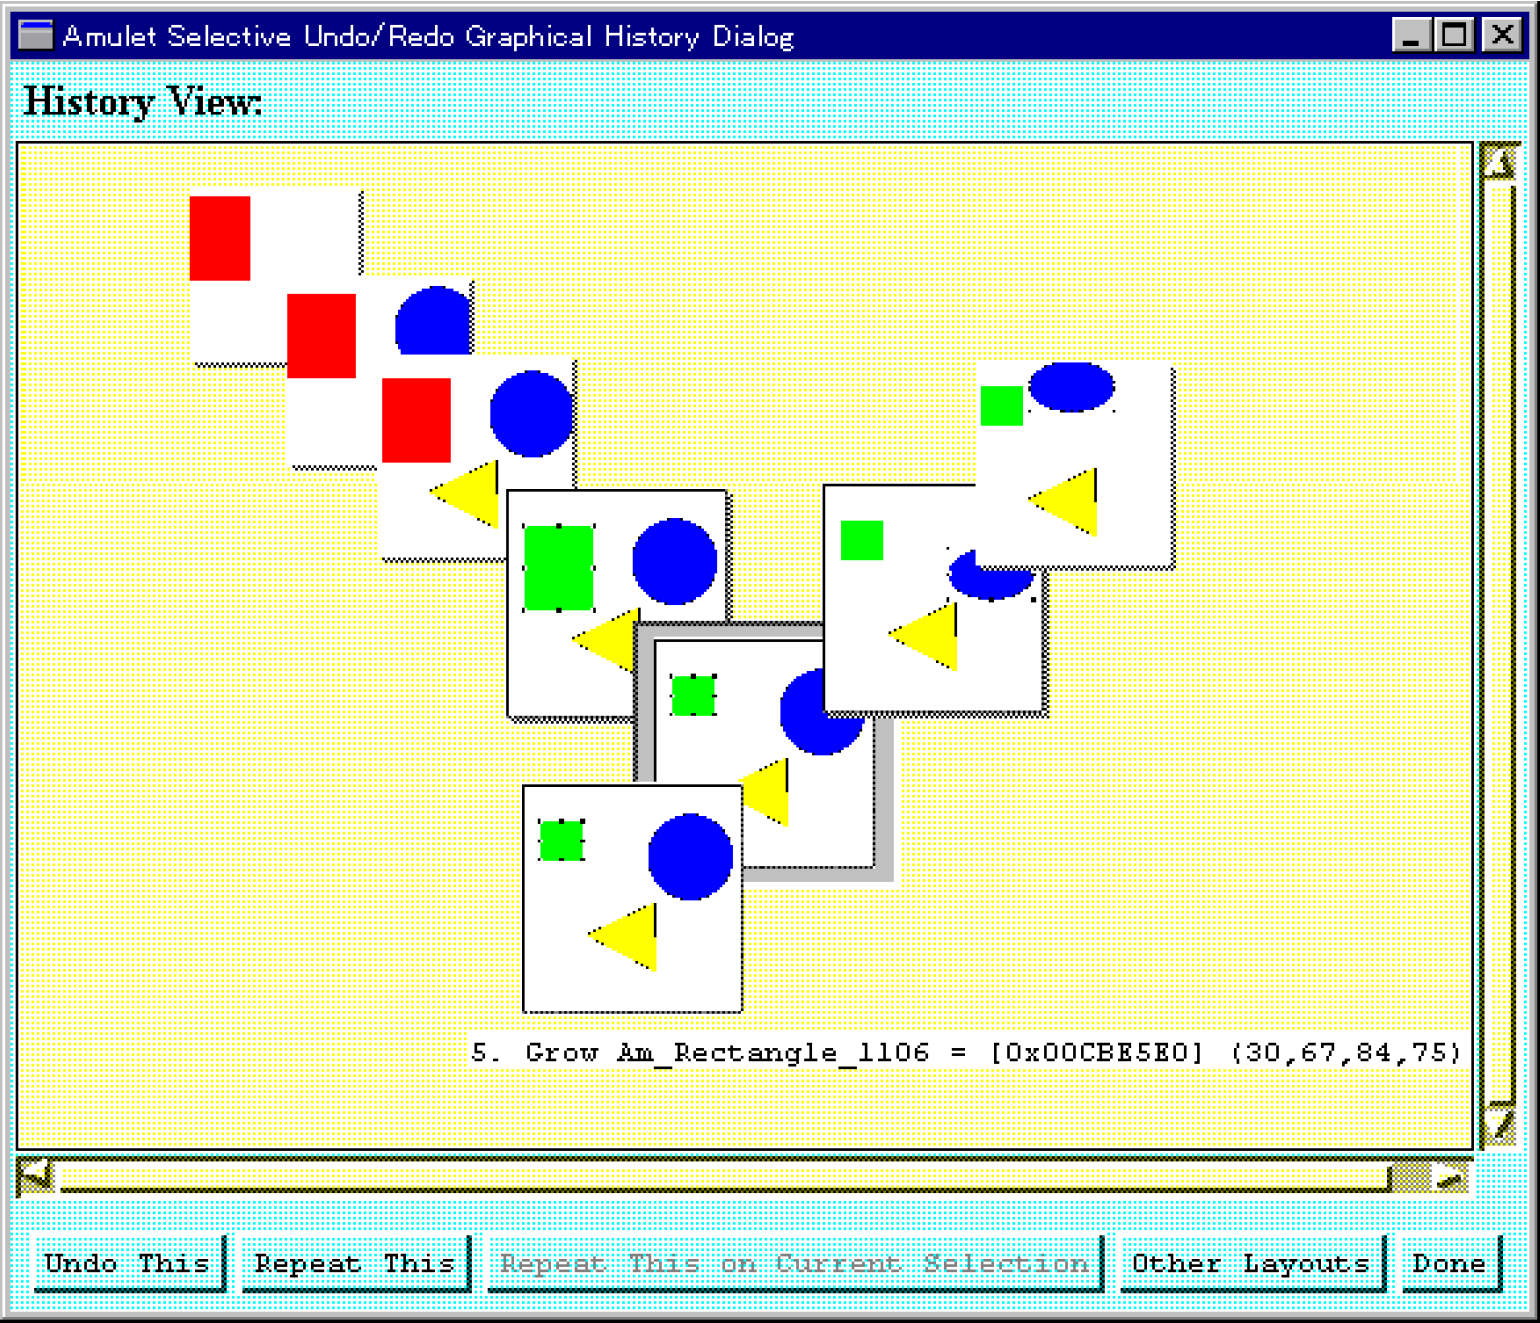
\includegraphics[width=.7\textwidth]{Perspective-View.png}
%%\caption{An example of using perspective view in provenance visualisation layout: further objects are smaller \cite{Meng1998}.}
%%\label{fig:Perspective-View}
%%\end{figure}
%
%%\subsubsection{Other Techniques}
%%Instead of displaying the history of actions in a temporal order, other factors can be used to reveal different aspects of the analysis process; for example, the flow of data retrieved during the course of the analysis is shown in the \textit{dependency graph} \cite{Kadivar2009} (Figure \ref{fig:Dependency-Graph}). The implemented system uses a scripting language to model the analysis process and each set of retrieved data is assigned to a variable; and thus, uses variable names to visualise the active data in each analysis step. However, this method may not be easy to apply to a generic non-scripting language system because it is not easy to visualise the difference between each set of data.
%%
%%\begin{figure}[ht]
%%\centering
%%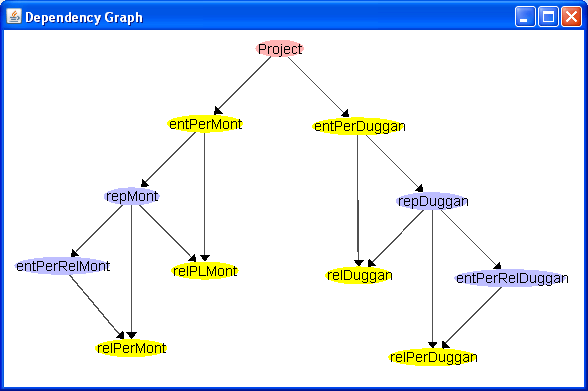
\includegraphics[width=.75\textwidth]{Dependency-Graph.png}
%%\caption{Dependency graph of the analysis session of a scenario from the novel \textit{The Day of the Jackal} \cite{Kadivar2009}. First, the analyst searches for person \textit{Montpellier} and the result is assigned to \textit{entPerMont}. Then, all reports related to Montepellier are fetched to \textit{repMont}. All persons mentioned in those reports are listed for further investigation (\textit{entPerRelMont}). The analyst notices on \textit{Duggan} and continues investigating that person. This is the flow that the analyst investigates the case; however, in the data perspective, after noticing Duggan, the analyst restarts the steps as he or she did with Montepellier. Therefore, in terms of data, Montepellier and Duggan are two independent branches in the data analysis tree.}
%%\label{fig:Dependency-Graph}
%%\end{figure}
%%
%%Another method to recall the analysis process is through the statistical usages of the system such as the most used visualisation tools and most investigated data objects \cite{Shrinivasan2009a}. This method provides a good overview of the analysis; however, it cannot show the sequence of actions performed during the analysis.
%
%\subsection{Utilising the Visualised Provenance}
%\label{sub:utilisation}
%The visualised provenance can be exploited to support the analytical reasoning process and collaboration.
%
%\subsubsection{Supporting the Analytical Reasoning Process}
%\paragraph{Recalling the Analysis Process}
%Provenance visualisation provides a visual overview of the analysis process. Therefore, it helps the analyst recall what has been done, and potentially reminds what is missing and what should be done. Provenance visualisation should not be a static picture of the past. In contrast, it should allow the analyst to freely navigate back to the desired state \cite{Derthick2001, Klemmer2002, Bavoil2005}. A state can be easily selected through the interface or with the help of \textit{search and filter} mechanism when there are too many recorded states. During the analysis process, users can take notes and tag keywords on visualisations; and all these metadata are subjects to search \cite{Shrinivasan2009a}. Moreover, VisTrails supports \textit{query-by-example} to find related visualisations \cite{Scheidegger2007}. Past states can be filtered to display periodically \cite{Klemmer2002} or based on a particular metadata such as authors \cite{Klemmer2002} and time \cite{Shrinivasan2009a}.
%
%\paragraph{Reusing the Performed Analyses}
%When reviewing the provenance, analysts can insert missing actions, remove undesired actions, and reapply past actions to a new dataset \cite{Derthick2001}. The past actions can also be modified directly by changing the command statements \cite{Kadivar2009}, the command parameters \cite{Gotz2010}, and the changing effects can be propagated along the history trail \cite{Ma1999}.
%
%Typically, in scientific visualisation, a visualisation is considered as a rendering result of many understandable parameters. Therefore, it is feasible to compare visualisations by measuring these sets of parameter values. VisTrails,  \cite{Bavoil2005}, a scientific visualisation workflow system, allows comparing and merging two visualisations into a new one. More specifically, \textit{set} operations including \textit{intersection}, \textit{union} and \textit{difference} can be employed to build the parameter set of the generated visualisation. In GraphTrail \cite{Dunne2012}, a information visualisation tool, it is still possible to merge visualisations in terms of data. The active dataset of each visualisation is mapped with a \textit{SQL statement}; thus, performing a SQL \textit{union} statement will result a new visualisation with the combined data of interest.
%
%\paragraph{Supporting Evidence in Constructing the Reasoning Process}
%As discussed in Section \ref{sub:reasoningprocess}, the reasoning process can be graphically documented inside the system. By capturing analytic provenance, we can attach the recorded visualisation to the reasoning evidence to support that artefact \cite{Shrinivasan2008}. Not only the visualisation but also could all the steps that the analyst performed to generate that visualisation be helpful.
%
%\subsubsection{Supporting Collaboration}
%\paragraph{Dissemination and Discussion}
%Visualisations can be annotated, captured and attached into the discussion forum to help peers understand the findings of author easier \cite{Heer2009}. Captured provenance can also be embedded into a formal analysis story to visually convey idea \cite{Eccles2007}. The embedded provenance should be interactive so that audience can examine and verify what the author wrote \cite{Pike2009a}. In asynchronous collaboration, each individual colleague can capture insight and submit them to a central repository. As a result, all peers can exploit other findings and facilitate the solving problem process \cite{Chen2011}.
%
%\paragraph{Presentation}
%Analytic provenance can also be exported for presentation purpose with various published formats. Outpost \cite{Klemmer2002}, a tangible interface for collaborative web site design, provides a \textit{print version} of annotated visualisations as a report. VisTrails \cite{Bavoil2005}, a scientific workflow and provenance management system, supports embedding the visualisation process into a paper through \textit{Latex} format. Image Graphs \cite{Ma1999}, a volume visualisation system, builds an \textit{animation} from selected key visualisations.
%
%%Chinchor and Pike propose four characteristics that a new generation analytical presentation should possess \cite{Chinchor2009}. The first characteristic is \textit{auditability}. The product needs to contain provenance information that provides both information of source data and analytic operations that were performed to generate it. The second characteristic is \textit{dynamic}. When data or any other inputs changes, the product should be updated automatically so that recipients can always work with the most up-to-date analysis. The third characteristic is \textit{interactivity}. The audience should be able to interact with the product to gain better understanding instead of just reading a static report. The fourth characteristic is \textit{context sensitivity}. The product should be sufficiently flexible to have different forms for people with different presentation needs.
%%
%%According to these four characteristics, the analytical presentations of Outpost, VisTrails and Image Graphs are auditable because they are composed from the captured provenance. The dynamic characteristic is not clearly mentioned in their work. However, these presentations are not interactive nor context-sensitive.